\subsection{Experimental setup}
\label{sec:setup}

\textbf{Drafters.} Every DFlash experiment starts from one pretrained checkpoint released for Qwen3-4B~\citep{chen2026dflash,yang2025qwen3}. It reads five target streams at zero-based layers 1, 9, 17, 25 and 33, has draft width 2{,}560 with $2560\times2560$ fusion blocks, and drafts a 16-token block from one anchor and 15 masked positions. Section~\ref{sec:eagle} additionally uses published EAGLE-3 checkpoints, which read three streams~\citep{li2025eagle3}. No draft transformer is ever trained.

\textbf{Targets.} In the \emph{fine-tuned} setting the target is a base model carrying a LoRA adapter that the released drafter has never seen~\citep{hu2022lora}: Qwen3-4B with a GSM8K, KiCad or NanoCoder adapter, and Qwen3-8B with a GSM8K or CodeAlpaca~\citep{chaudhary2023codealpaca} adapter, each merged into the frozen target before inference. In the \emph{replaced} setting the target is a different model from the one the drafter was built for. We evaluate four such transfers, named by the target they accelerate and the model the drafter came from: Qwen3-8B from Qwen3-4B, Qwen3-4B from Qwen3-8B, Llama3.1-8B from Qwen3-4B, and Llama3.2-3B from Llama3.1-8B~\citep{grattafiori2024llama3}. Llama3.1-8B from Qwen3-4B is the only pair whose tokenizers differ, so it also uses the proposal bridge of Section~\ref{sec:method-generation}. Maps are square $2560\times2560$ when the target keeps the drafter's feature width, giving 32.8M trained parameters, and $2560\times4096$ when accelerating Qwen3-8B, giving 52.4M.

\textbf{Reference drafters.} Each setting has one meaningful reference, and we name it explicitly wherever a number is relative to it. For a fine-tuned target the reference is the \emph{unadapted drafter}, the released checkpoint run against the fine-tuned target with no adaptation. It is the honest reference because no drafter exists for a LoRA variant, so this is what a deployment would otherwise use. For a replaced target the reference is the \emph{native drafter}, a drafter trained specifically for the target being accelerated. This is the demanding reference, because matching it means reaching the quality of target-specific drafter training without doing any. Autoregressive decoding, the target with no drafter at all, is the common denominator for both.

\textbf{Datasets and benchmarks.} Transfer experiments use MATH test~\citep{hendrycks2021math}, GSM8K test~\citep{cobbe2021gsm8k}, pinned LiveCodeBench releases~\citep{jain2024livecodebench} and single-turn instructions derived from UltraFeedback~\citep{cui2024ultrafeedback}, reported as Math, GSM8K, Code and Chat. Fine-tuned-target experiments evaluate on held-out prompts from the adapter's own domain. Every reported cell uses 128 held-out prompts with a 2{,}048-token response cap, except KiCad at 8{,}192.

\textbf{Metrics.} RelaySpec changes only the drafter's inputs and leaves the target and its acceptance rule untouched, so we report acceleration rather than task quality. \emph{Speedup} is mean per-request throughput divided by that of autoregressive decoding of the same target on the same prompts, so autoregressive decoding is $1.00\times$ by definition. \emph{Acceptance length} $\tau$ is pooled emitted tokens per verification step and includes the correction token, so its floor is one. Section~\ref{sec:serving} additionally reports \emph{aggregate throughput}, total returned tokens divided by workload wall time including drain. These statistics weight requests differently and we never mix them inside one comparison. Where an ablation must choose one configuration, we select by the harmonic mean of its per-workload speedups rather than their average, because the harmonic mean of ratios is pulled down by the smallest entry and so will not let a configuration hide one weak workload behind a favourable average. We use it only for those selections.

\textbf{Implementation details.} For a fine-tuned target we generate 4{,}096 responses with that target, cache its hidden states, sample 32 anchors per example, and train one epoch, which is 512 optimizer updates at global batch 8 with AdamW~\citep{loshchilov2019adamw} at learning rate $10^{-4}$. For a replaced target we reuse 16{,}384 saved NuminaMath~\citep{li2024numinamath} trajectories, supervise a fixed 25\% of prompt and response positions, and train three epochs, which is 6{,}144 updates at learning rate $10^{-3}$. Both use seed 42 on two L40S GPUs with FP32 trainable maps over a frozen BF16 model, and both export the folded projection in BF16. Single-request measurements use the Transformers library~\citep{wolf2020transformers} on one L40S with greedy non-thinking decoding, CUDA-synchronized timing and warmup excluded. Serving measurements use vLLM 0.28.0~\citep{kwon2023vllm} with batch-invariant operations and FlashAttention kernels~\citep{dao2023flashattention2}. We report vLLM numbers throughout; other serving stacks such as SGLang~\citep{zheng2024sglang} implement speculative decoding differently and are not directly comparable. In the selected single-request comparisons the unadapted, native and adapted drafters returned identical output sequences on all 128 prompts per workload, so those ratios are not confounded by output length. Under vLLM the sequences can diverge and we treat those numbers as descriptive.

\subsection{Main results}
\label{sec:main-results}
Table~\ref{tab:main} reports every target, workload and reference in one place. Two conclusions follow from it.

\begin{table}[t]
\centering
\caption{Complete single-request results. AR is the measured autoregressive tokens per second for that target on that workload, the common $1.00\times$ baseline for every speedup in the row. Speedup is mean per-request throughput divided by AR. $\tau$ is average acceptance length including the correction token. The reference for a fine-tuned target is the released drafter used with no adaptation, so $\times$ref above 1 is an improvement over what a deployment would otherwise run. The reference for a replaced target is a drafter trained for that target, so $\times$ref near 1 means RelaySpec matches target-specific drafter training without performing any. A target written $A\leftarrow B$ is target $A$ accelerated by a drafter built for $B$. Bold marks $\times$ref at or above parity.}
\label{tab:main}
\small
\setlength{\tabcolsep}{4.2pt}
\begin{tabular}{llrrrrrr}
\toprule
& & & \multicolumn{2}{c}{RelaySpec} & \multicolumn{2}{c}{Reference drafter} & \\
\cmidrule(lr){4-5}\cmidrule(lr){6-7}
Target $\leftarrow$ drafter & Workload & AR & Speedup & $\tau$ & Speedup & $\tau$ & $\times$ref \\
\midrule
\multicolumn{8}{l}{\emph{Fine-tuned target. Reference is the released drafter, used unadapted.}} \\
Qwen3-4B + GSM8K LoRA & GSM8K & 38.81 & 4.63$\times$ & 5.99 & 3.32$\times$ & 4.47 & \textbf{1.40} \\
Qwen3-4B + KiCad LoRA & KiCad & 38.42 & 8.13$\times$ & 11.26 & 4.39$\times$ & 5.99 & \textbf{1.85} \\
Qwen3-4B + NanoCoder LoRA & NanoCoder & 39.01 & 4.40$\times$ & 5.55 & 3.87$\times$ & 5.11 & \textbf{1.14} \\
Qwen3-8B + GSM8K LoRA & GSM8K & 37.89 & 4.59$\times$ & 6.35 & 3.40$\times$ & 4.76 & \textbf{1.35} \\
Qwen3-8B + CodeAlpaca LoRA & CodeAlpaca & 37.56 & 4.32$\times$ & 5.63 & 4.07$\times$ & 5.62 & \textbf{1.06} \\
\midrule
\multicolumn{8}{l}{\emph{Replaced target. Reference is a drafter trained for the target being accelerated.}} \\
Qwen3-8B $\leftarrow$ Qwen3-4B & Math & 37.84 & 5.82$\times$ & 7.98 & 5.81$\times$ & 8.21 & \textbf{1.00} \\
 & GSM8K & 37.76 & 4.68$\times$ & 6.24 & 4.71$\times$ & 6.48 & 0.99 \\
 & Code & 37.50 & 3.40$\times$ & 4.74 & 4.04$\times$ & 5.64 & 0.84 \\
 & Chat & 35.09 & 2.31$\times$ & 2.89 & 2.55$\times$ & 3.32 & 0.90 \\
\addlinespace[1pt]
Qwen3-4B $\leftarrow$ Qwen3-8B & Math & 39.42 & 5.49$\times$ & 7.66 & 5.70$\times$ & 8.09 & 0.96 \\
 & GSM8K & 39.72 & 4.27$\times$ & 5.99 & 4.46$\times$ & 6.34 & 0.96 \\
 & Code & 39.60 & 3.30$\times$ & 4.89 & 4.34$\times$ & 6.26 & 0.76 \\
 & Chat & 40.48 & 2.01$\times$ & 2.83 & 2.36$\times$ & 3.36 & 0.85 \\
\addlinespace[1pt]
Llama3.1-8B $\leftarrow$ Qwen3-4B & Math & 41.00 & 2.97$\times$ & 4.63 & 3.17$\times$ & 5.12 & 0.94 \\
 & GSM8K & 41.11 & 2.21$\times$ & 3.23 & 3.10$\times$ & 4.42 & 0.71 \\
 & Code & 40.79 & 1.98$\times$ & 3.05 & 3.00$\times$ & 4.52 & 0.66 \\
 & Chat & 40.96 & 1.48$\times$ & 2.06 & 2.79$\times$ & 3.95 & 0.53 \\
\bottomrule
\end{tabular}
\setlength{\tabcolsep}{6pt}
\end{table}

\textbf{Adapting a fine-tuned target's features recovers a large share of lost drafting quality.} Training only the five maps improves every adapter at both target scales, from $+6\%$ on CodeAlpaca to $+85\%$ on KiCad, and raises acceptance length in every cell. The size of the gain tracks acceptance rather than any change to the inference path: KiCad nearly doubles acceptance length, from 5.99 to 11.26, and reaches $8.13\times$ autoregressive throughput, whereas CodeAlpaca moves from 5.62 to 5.63 and gains little. The improvement is therefore a function of how far the adapter moved the target away from what the drafter expects, which is exactly the quantity the method is designed to absorb.

\textbf{A drafter can be moved to a different target model and still approach one built for it.} Every transfer accelerates its target on every workload, so a frozen draft transformer can be driven by mapped features from a model it was never trained on, including across a family and a tokenizer boundary. Within the Qwen3 family the maps reach $1.002\times$ and $0.994\times$ of a native drafter on Math and GSM8K when moving up in scale, without any target-specific drafter training. Recovery is lower on Code and Chat, and lower again across families, so we report the setting as effective within a family and partial across one.

Table~\ref{tab:llama-transfer} reports a fifth transfer, a Llama3.1-8B drafter reused for Llama3.2-3B. Four trained input maps reach $2.35\times$ autoregressive throughput on Math and above $1.6\times$ on every workload.

\begin{table}[t]
\centering
\caption{Llama3.1-8B drafter reused for Llama3.2-3B. Speedup is relative to autoregressive decoding (AR), the same $1.00\times$ baseline convention as Table~\ref{tab:main}.}
\label{tab:llama-transfer}
\small
\begin{tabular}{lrrr}
\toprule
Workload & AR (tok/s) & Speedup & $\tau$ \\
\midrule
Math & 61.90 & 2.35$\times$ & 4.78 \\
GSM8K & 64.45 & 2.18$\times$ & 4.16 \\
Code & 63.09 & 1.88$\times$ & 3.44 \\
Chat & 64.73 & 1.61$\times$ & 2.97 \\
\bottomrule
\end{tabular}
\end{table}

\FloatBarrier
\subsection{Ablation studies}
\label{sec:ablations}
We ablate the three decisions that define the method: where the trained parameters sit, which objective trains them, and how much capacity and supervision they need. Each ablation holds data, schedule and evaluation fixed and changes one element.

\subsubsection{Where the trained parameters sit}
\label{sec:ablation-placement}
RelaySpec trains one map per feature stream and then folds those maps into the fusion block in front of which they sit. Because the folded result is a single matrix, the natural objection is that the factorization is irrelevant and any trainable matrix of the same size would do. Table~\ref{tab:ablation-placement} tests that, against four alternatives:

\begin{itemize}\itemsep1pt\parskip0pt
\item \textbf{Single fused projection.} One matrix of the same total size, trained in place of the five maps and initialized to exactly the function the five maps start from. This is the decisive control, since it differs from RelaySpec only in being unfactorized.
\item \textbf{Draft-transformer LoRA.} A rank-128 LoRA on the attention and MLP projections inside the draft blocks. This trains the drafter's body instead of its inputs, and is the established alternative that RelaySpec is meant to replace.
\item \textbf{Single joint map.} One dense matrix over all five concatenated streams, which permits mixing between streams at five times the parameters.
\item \textbf{Rank-$r$ maps.} Each whole map is replaced by a rank-$r$ product, rather than adding a low-rank correction to a retained full map.
\end{itemize}

\begin{table}[t]
\centering
\caption{Where the trained parameters sit, for fine-tuned Qwen3-4B targets under a matched accept-until-fail objective, 4{,}096 examples and 32 anchors. Values are percent gain in mean throughput over the unadapted drafter. HM is the harmonic mean of the corresponding speedup ratios and is the selection criterion. Best in each column in bold.}
\label{tab:ablation-placement}
\small
\begin{tabular}{lrrrrr}
\toprule
Trained object & Parameters & GSM8K & KiCad & NanoCoder & HM \\
\midrule
Five per-stream maps (RelaySpec) & 32.8M & $\mathbf{+37.6}$ & $+89.5$ & $+8.1$ & \textbf{1.376} \\
Single fused projection & 32.8M & $+32.4$ & $+44.5$ & $+8.2$ & 1.265 \\
Draft-transformer LoRA, rank 128 & 36.7M & $+36.4$ & $+75.5$ & $\mathbf{+9.8}$ & 1.355 \\
Single joint map over all streams & 163.8M & $+24.3$ & $\mathbf{+88.4}$ & $-7.0$ & 1.244 \\
Rank-128 maps & 3.3M & $+3.2$ & $+58.4$ & $-28.8$ & 0.999 \\
Rank-56 maps & 1.4M & $-21.9$ & $+35.1$ & $-49.3$ & 0.751 \\
Rank-28 maps & 0.7M & $-43.1$ & $+12.8$ & $-62.5$ & 0.565 \\
\bottomrule
\end{tabular}
\end{table}

\textbf{What this shows.} For scale, the unadapted drafter used as the 0\% reference here already reaches $3.3\times$ to $4.4\times$ autoregressive decoding before any adaptation (Table~\ref{tab:main}), so every percentage below is the further gain adaptation adds on top of that autoregressive speedup, not the whole story. The factorization does the work, not the parameter count. With identical parameters and an identical starting function, the single fused projection reaches a harmonic mean of 1.265 against 1.376 for the five maps and loses 45 points of gain on KiCad. The same contrast appears when transferring to Qwen3-8B, where under a matched objective the single fused projection reaches $0.365\times$ the native drafter on Math while the five maps reach $0.884\times$. Keeping one map per stream therefore changes what the optimizer can reach, even though the two parameterizations describe the same functions after folding and export as the same matrix. This is the behaviour that structural re-parameterization predicts, where a training-time factorization that merges away at inference still improves the trained result~\citep{huo2026repspec}. Replacing each whole map by a low-rank product degrades monotonically, and the two smallest ranks fall below the unadapted drafter, because replacing the map discards its ability to pass the original feature through rather than merely limiting the learned correction. Draft-transformer LoRA is competitive and wins on NanoCoder, so we do not claim that adapting inputs beats adapting the body on every workload. Its cost is that the draft transformer is no longer shared, which Section~\ref{sec:serving} shows is what makes the method useful in deployment.

\subsubsection{Which objective trains the maps}
\label{sec:ablation-objective}
The two settings start from different places. With a fine-tuned target the maps start at the identity and the drafter already reads a usable interface, so what remains is to predict a shifted token distribution. With a replaced target the maps start random and possibly rectangular, so the interface itself is not yet usable. Table~\ref{tab:ablation-objective} compares the candidates and selects by harmonic mean.

\begin{table}[t]
\centering
\caption{Which objective trains the maps. The upper block reports throughput relative to the unadapted drafter for fine-tuned Qwen3-4B targets. The lower block reports throughput relative to the native Qwen3-8B drafter for transfer from Qwen3-4B, on the matched 8{,}192-example fits. MSE50 and MSE100 supervise that fraction of prompt and response positions. Best in each column in bold. HM is the selection criterion.}
\label{tab:ablation-objective}
\small
\begin{tabular}{llrrrrr}
\toprule
Setting & Objective & \multicolumn{4}{c}{Workload} & HM \\
\midrule
 & & GSM8K & KiCad & NanoCoder & & \\
\cmidrule(lr){3-5}
Fine-tuned & Accept-until-fail & \textbf{1.376} & 1.895 & \textbf{1.081} & & \textbf{1.376} \\
 & Decaying cross-entropy & 1.368 & \textbf{1.935} & 1.031 & & 1.353 \\
 & Reconstruction, MSE50 & 1.011 & 1.191 & 0.977 & & 1.052 \\
\midrule
 & & Math & GSM8K & Code & Chat & \\
\cmidrule(lr){3-6}
Replaced & Reconstruction, MSE100 & 0.998 & \textbf{0.990} & 0.828 & \textbf{0.891} & \textbf{0.921} \\
 & Reconstruction, MSE50 & \textbf{0.999} & 0.975 & \textbf{0.832} & 0.888 & 0.919 \\
 & Decaying cross-entropy & 0.886 & 0.919 & 0.406 & 0.573 & 0.623 \\
 & Accept-until-fail & 0.884 & 0.911 & 0.385 & 0.558 & 0.604 \\
\bottomrule
\end{tabular}
\end{table}

\textbf{What this shows.} The harmonic mean makes the selection unambiguous and shows why an average would not. For a fine-tuned target the two token objectives are nearly tied on the arithmetic mean, 1.451 for accept-until-fail against 1.445 for decaying cross-entropy, because the latter's strong KiCad result offsets its weak NanoCoder result. The harmonic mean separates them, 1.376 against 1.353, because it refuses to let the 1.031 NanoCoder entry be averaged away, and a deployment meets that workload. Reconstruction on the same fine-tuned targets reaches only 1.052, behind both token objectives and, on NanoCoder, behind the unadapted drafter itself, because it trains the maps toward the base model's features rather than toward the tokens the adapted target actually produces. We therefore select accept-until-fail for fine-tuned targets. For a replaced target the ordering reverses and becomes decisive: both reconstruction variants exceed 0.918 while the best token objective reaches only 0.623, and the gap comes almost entirely from Code and Chat, where token supervision collapses to 0.406 and 0.573. We select reconstruction there. Among the two token objectives the harmonic mean prefers decaying cross-entropy for a replaced target, the reverse of the fine-tuned ordering, so neither token objective dominates across settings and the pairing of objective to setting is doing real work in both directions. Doubling supervised positions from MSE50 to MSE100 moves the harmonic mean by 0.002 while tripling the fitting time, so the deployed recipe supervises a quarter of positions. One qualification: the reconstruction runs use learning rate $10^{-3}$ and the token runs $10^{-4}$, so these compare complete recipes rather than losses at one fixed setting.

Two further checks support this choice without changing it. First, on a separate matched architecture (a single low-rank fusion update rather than the five per-stream maps, held fixed to isolate the loss), plain uniform cross-entropy, the DFlash decaying weighting, and accept-until-fail were compared under identical data and schedule on NanoCoder: accept-until-fail reaches $1.072\times$ autoregressive decoding against $1.046\times$ for uniform cross-entropy and $1.047\times$ for decaying cross-entropy, a $2.4\%$ gain over uniform weighting that decaying weighting does not reproduce. This confirms that the prefix-aware accept-until-fail weighting, not merely having some position-dependent weighting, is what improves throughput. Second, for a fine-tuned target the training responses do not need to come from the fine-tuned target itself: fitting the same architecture from the base model's own generations reaches $1.001\times$ the throughput of fitting from the fine-tuned target's generations on the fine-tuned target's evaluation prompts, with a paired 95\% interval of $[0.995, 1.007]$ that contains 1. The gain therefore reflects adaptation to the workload distribution rather than a fit to the fine-tuned target's specific outputs, which is why we generate training responses with whichever target will be evaluated rather than requiring matched labeled data.

\subsubsection{Whether the maps need to be nonlinear}
\label{sec:ablation-capacity}
The maps are linear because a linear map changes the feature width and still folds into the fusion projection. To test whether that costs accuracy, we add a parallel nonlinear branch to each map, so stream $i$ contributes $W_ih_i+B_i\operatorname{SiLU}(A_ih_i)$~\citep{elfwing2018silu}, with $A_i$ reducing to 256 coordinates and $B_i$ initialized to zero. Training therefore starts at exactly the linear solution and departs from it only if that lowers the loss. The branch raises trained parameters from 32.8M to 39.3M for a fine-tuned target and from 52.4M to 60.9M for transfer, and unlike the linear map it cannot be folded away before inference. Table~\ref{tab:ablation-capacity} holds data, objective and schedule fixed within each setting.

\begin{table}[t]
\centering
\caption{Whether the maps need to be nonlinear. Values are mean tokens per second and acceptance length under matched data, objective and schedule. The nonlinear alternative carries 16 to 20 percent more parameters and remains an active computation at inference. Best in each row in bold.}
\label{tab:ablation-capacity}
\small
\begin{tabular}{llrrrrr}
\toprule
& & \multicolumn{2}{c}{Tokens/s} & & \multicolumn{2}{c}{$\tau$} \\
\cmidrule(lr){3-4}\cmidrule(lr){6-7}
Setting & Workload & Linear & Nonlinear & Change & Linear & Nonlinear \\
\midrule
Fine-tuned & GSM8K & \textbf{179.83} & 177.94 & $-1.05\%$ & \textbf{5.988} & 5.953 \\
 & KiCad & 312.47 & \textbf{321.76} & $+2.97\%$ & 11.256 & \textbf{11.411} \\
 & NanoCoder & \textbf{171.73} & 169.74 & $-1.16\%$ & \textbf{5.552} & 5.520 \\
\midrule
Replaced & Math & \textbf{220.26} & 215.71 & $-2.07\%$ & \textbf{7.984} & 7.980 \\
 & GSM8K & \textbf{176.87} & 174.56 & $-1.31\%$ & 6.242 & \textbf{6.257} \\
 & Code & 127.61 & \textbf{128.41} & $+0.63\%$ & 4.739 & \textbf{4.782} \\
 & Chat & \textbf{80.93} & 80.78 & $-0.20\%$ & 2.887 & \textbf{2.902} \\
\bottomrule
\end{tabular}
\end{table}

\textbf{What this shows.} The nonlinear branch is given every advantage, since it starts from the linear solution, carries more parameters and is selected by the optimizer only if it lowers the loss. It nevertheless changes throughput by between $-2.07\%$ and $+2.97\%$, leaves acceptance length almost unchanged, and is behind the linear map on five of the seven workloads. The linear form is therefore not a concession made for foldability. It is at least as accurate here and additionally collapses to one fixed matrix before inference. With differences of this size and one timed pass per cell we claim only that this nonlinear interface does not pay for itself.

\subsubsection{How much supervision the maps need}
\label{sec:ablation-budget}
Both recipes use small budgets, which raises three questions: how little data the maps actually need, whether the larger budgets are saturated, and whether draft-transformer LoRA would overtake the maps given more data. Figure~\ref{fig:scaling} varies the supervision axes for both settings from 16 to 16{,}384 examples, spanning three orders of magnitude.

\begin{figure}[t]
    \centering
    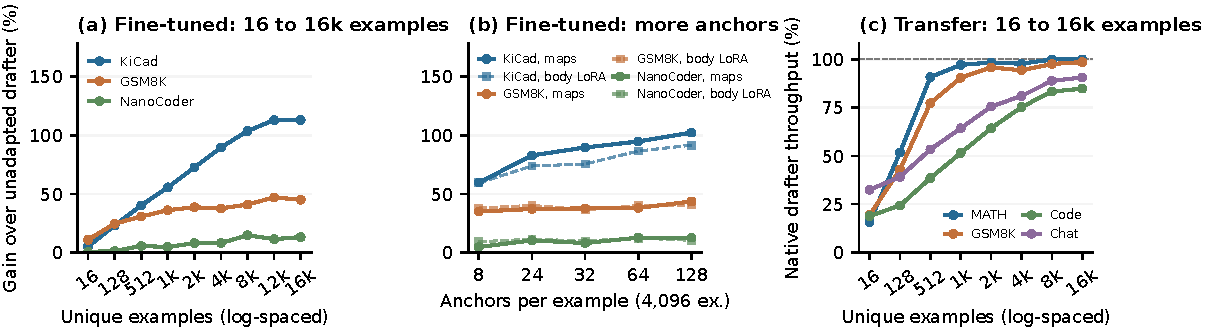
\includegraphics[width=\linewidth]{figures/relayspec_scaling.pdf}
    \caption{Supervision budget in both settings, from 16 to 16{,}384 training examples. (a) and (c) share a log-spaced example axis; (b) fixes examples at 4{,}096 and varies anchors per example. (a) and (b) use fine-tuned Qwen3-4B targets with the accept-until-fail objective, where solid lines train the five interface maps and dashed lines train a rank-128 LoRA inside the draft transformer. (c) transfers the Qwen3-4B drafter to Qwen3-8B with the reconstruction objective and plots throughput as a percentage of the native Qwen3-8B drafter. Adaptation is already effective at 16 examples and speedup keeps improving with supervision without saturating at the largest budget measured.}
    \label{fig:scaling}
\end{figure}


\textbf{What this shows.} Adaptation is effective from as few as 16 examples. On a fine-tuned target with only 16 examples the maps already recover part of the gap, and throughput then rises smoothly and without saturating out to 16{,}384 examples: GSM8K goes from $+10.8\%$ to $+45.0\%$, KiCad from $+5.0\%$ to $+113.0\%$, and NanoCoder from $+0.5\%$ to $+13.1\%$. Recovery of the native drafter under transfer follows the same pattern, rising from 15.6\% to 99.9\% on Math, 19.4\% to 98.5\% on GSM8K, 18.9\% to 84.8\% on Code, and 32.5\% to 90.5\% on Chat, so the workloads that transfer least well at large budgets are also the ones that still have the most to gain from more data. Because neither curve has saturated at the largest budget measured, the main results in Table~\ref{tab:main} are conservative operating points rather than ceilings. Panel (b) shows the two curves crossing on the anchor axis: at the smallest anchor budget the maps lead draft-transformer LoRA clearly on KiCad, $+59.7\%$ against $+75.5\%$ in the opposite direction, and at 128 anchors the two are within a few points of each other on every domain. Interface adaptation is therefore the more data-efficient choice at the low end of the supervision budget, and its advantage is largest in exactly the regime the method targets, where a new target variant must be supported from very little data.

\subsection{Generalization to a second drafter family}
\label{sec:eagle}
The construction should not depend on DFlash. We repeat both settings on published EAGLE-3 checkpoints, which read three target streams and draft one token at a time rather than filling a masked block, pairing each setting with the objective that Section~\ref{sec:ablation-objective} selected for it. Table~\ref{tab:eagle} reports the result.

\begin{table}[t]
\centering
\caption{Generalization to EAGLE-3, using three input maps. Token supervision is used for a fine-tuned target and reconstruction for a replaced one, following the selection in Section~\ref{sec:ablation-objective}. The reference is the unadapted EAGLE-3 drafter for the fine-tuned block and a published EAGLE-3 drafter native to Qwen3-8B for the replaced block. Best in each row in bold. Acceptance uses EAGLE-3's upstream counters and is not comparable with the DFlash tables.}
\label{tab:eagle}
\small
\begin{tabular}{llrrrrr}
\toprule
& & \multicolumn{2}{c}{Tokens/s} & & \multicolumn{2}{c}{$\tau$} \\
\cmidrule(lr){3-4}\cmidrule(lr){6-7}
Setting & Workload & Reference & RelaySpec & $\times$ref & Reference & RelaySpec \\
\midrule
Fine-tuned Qwen3-4B, & GSM8K & 71.19 & \textbf{120.35} & \textbf{1.69} & 3.347 & \textbf{5.695} \\
token supervision & NanoCoder & 81.77 & \textbf{119.30} & \textbf{1.46} & 3.852 & \textbf{5.668} \\
 & KiCad & 73.82 & \textbf{151.86} & \textbf{2.06} & 3.794 & \textbf{7.363} \\
\midrule
Qwen3-8B from Qwen3-4B, & Math & 72.18 & \textbf{77.99} & \textbf{1.08} & 3.627 & \textbf{3.638} \\
reconstruction & GSM8K & 75.58 & \textbf{80.59} & \textbf{1.07} & 3.713 & \textbf{3.840} \\
 & Code & 63.88 & \textbf{65.53} & \textbf{1.03} & \textbf{3.351} & 3.293 \\
 & Chat & 61.82 & \textbf{63.41} & \textbf{1.03} & \textbf{3.186} & 3.136 \\
\bottomrule
\end{tabular}
\end{table}

\textbf{What this shows.} Adapting the inputs of a frozen EAGLE-3 drafter improves it in both settings, by 45.9\% to 105.7\% on fine-tuned targets and above a purpose-built Qwen3-8B EAGLE-3 drafter on all four transfer workloads. Against autoregressive decoding of the same fine-tuned target, RelaySpec reaches $3.82\times$ on GSM8K, $3.75\times$ on NanoCoder and $5.00\times$ on KiCad, against $2.26\times$, $2.57\times$ and $2.43\times$ for the unadapted EAGLE-3 drafter. The objective selection also replicates, which is the stronger result. Training the same three maps by reconstruction on the fine-tuned targets, so that they reproduce the base model's features instead of predicting the adapted target's tokens, gives 71.89, 75.34 and 78.70 tokens per second, a 7.9\% regression on NanoCoder and almost no change on GSM8K. Token supervision instead gives 120.35, 119.30 and 151.86 on the same targets and prompts, between 58\% and 93\% faster. Pairing the objective to the setting is therefore not a DFlash artifact: it holds on a different draft architecture with a different drafting procedure. Two qualifications apply. Our recurrent token objective adapts the accept-until-fail rule to a sequential drafter and is not the masked-block implementation used for DFlash, so this transfers the rule rather than the code. And unlike the DFlash comparisons the EAGLE-3 runs do not return identical sequences, so we report throughput and acceptance rather than summed latency.

\subsection{Serving many targets from one drafter}
\label{sec:serving}
Because the draft transformer is never trained, several adapted targets can share one copy of it, with only a small matrix differing between them. This is what draft-transformer LoRA gives up. Figure~\ref{fig:serving} measures the deployment on a vLLM server holding one target backbone and one draft backbone with three LoRA targets and frozen route assignments.

\begin{figure}[t]
    \centering
    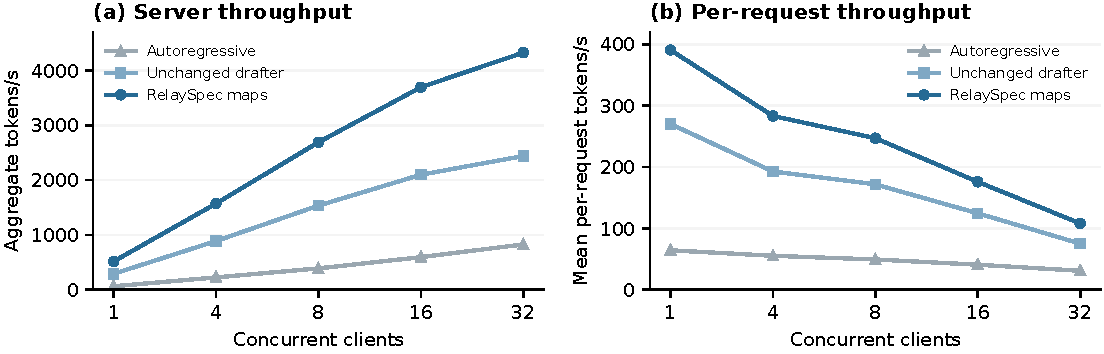
\includegraphics[width=\linewidth]{figures/relayspec_serving.pdf}
    \caption{One Qwen3-4B target backbone and one draft backbone serving three LoRA targets under vLLM on a single L40S, 384 requests with frozen route assignments. (a) aggregate throughput, total returned tokens divided by workload wall time including drain. (b) mean per-request throughput. The adapted drafter leads on server throughput at every concurrency, while per-request throughput falls with load for all three methods.}
    \label{fig:serving}
\end{figure}


\textbf{What this shows.} The single-request gains survive batching. Aggregate server throughput is higher for the adapted drafter at every concurrency measured, reaching 4{,}324 tokens per second against 2{,}440 for the unadapted drafter and 828 for autoregressive decoding at 32 clients, while acceptance length stays near 10.5 against 5.8. Panel (b) shows why both conventions must be reported: mean per-request throughput falls with load for all three methods even as server throughput rises, so a per-request number cannot stand in for a serving number. One pooled set of maps trained on the union of three domains reaches 98.9\% to 99.6\% of three separately trained sets across two repeats, so a deployment need not even hold one adapter per target. This is the practical form of the reuse question that motivates target-independent drafting~\citep{an2026pard2}. The advantage is not unbounded: on a Qwen3-8B server the adapted drafter leads at 1, 4 and 8 clients but falls within 4\% of the native drafter at 16 and 32 clients, because at high concurrency the bottleneck moves away from acceptance length.

\textbf{Concurrent serving across transfers.} The same question arises for a replaced target: does the transferred drafter still help once requests are batched under vLLM? Table~\ref{tab:transfer-serving} reports aggregate throughput at 16 concurrent clients for the three transfers with a published native drafter. Batching reproduces the single-request ordering of Table~\ref{tab:main} rather than changing it. On the transfer with the strongest single-request recovery, Qwen3-8B accelerated by the Qwen3-4B drafter, the mapped drafter leads on Math and GSM8K and trails narrowly on Code and Chat. On the reverse and cross-family transfers, where single-request recovery was already weaker, the mapped drafter trails the native drafter under concurrency on every workload, most on the cross-family Llama3.1-8B transfer. On the Llama3.2-3B transfer of Table~\ref{tab:llama-transfer}, the same server configuration reaches $2.53\times$, $3.08\times$, $1.71\times$ and $1.77\times$ autoregressive throughput on Math, GSM8K, Code and Chat at 16 clients.

\begin{table}[t]
\centering
\caption{Aggregate vLLM throughput at 16 concurrent clients, total returned tokens divided by workload wall time including drain. Bold marks the higher of native and mapped.}
\label{tab:transfer-serving}
\small
\begin{tabular}{llrrr}
\toprule
Target $\leftarrow$ drafter & Workload & Native (tok/s) & Mapped (tok/s) & Mapped/native \\
\midrule
Qwen3-8B $\leftarrow$ Qwen3-4B & Math & 2524.31 & \textbf{2716.26} & 1.076 \\
 & GSM8K & 2207.43 & \textbf{2262.03} & 1.025 \\
 & Code & \textbf{1748.19} & 1548.47 & 0.886 \\
 & Chat & \textbf{1091.14} & 1065.93 & 0.977 \\
\midrule
Qwen3-4B $\leftarrow$ Qwen3-8B & Math & \textbf{4482.42} & 3710.76 & 0.828 \\
 & GSM8K & \textbf{3160.99} & 3078.87 & 0.974 \\
 & Code & \textbf{2840.15} & 2002.79 & 0.705 \\
 & Chat & \textbf{1888.69} & 1431.21 & 0.758 \\
\midrule
Llama3.1-8B $\leftarrow$ Qwen3-4B & Math & \textbf{1894.99} & 1046.94 & 0.553 \\
 & GSM8K & \textbf{1354.50} & 853.13 & 0.630 \\
 & Code & \textbf{1296.83} & 636.97 & 0.491 \\
 & Chat & \textbf{1440.04} & 524.40 & 0.364 \\
\bottomrule
\end{tabular}
\end{table}

\textbf{Memory and GPU usage.} We measured post-request allocated and reserved GPU memory on the same T1 serving cells above. Allocated memory rises from 30.5914 GiB for the native drafter to 30.9190 GiB for the mapped drafter, a constant 0.33 GiB increase regardless of workload or concurrency; reserved memory shows the same small, workload-independent gap. This matches expectation: the trained maps add 52.4 million BF16 parameters to an 8-billion-parameter target and a several-billion-parameter draft transformer, so the memory cost of adaptation is negligible relative to the models it accelerates, and it does not grow with client count.

\subsection{Comparison with published systems}
\label{sec:related-work-compare}
The reports also include a public-runtime comparison of an earlier single-projection version of this interface against two published drafters that reuse or steer a fixed prediction network: PARD, which reuses a released parallel drafter with no new target-specific fitting~\citep{an2026pard}, and SD$^2$, evaluated in its frozen-drafter configuration, which steers a pretrained autoregressive drafter through injected features~\citep{berdoz2026steering}. All three ran on the same 128 MATH development questions with a 2{,}048-token cap, each reported against its own runtime's autoregressive baseline because the systems differ in precision, attention backend and supporting libraries. Table~\ref{tab:public-runtime} reports the result.

\begin{table}[t]
\centering
\caption{Public-runtime comparison on 128 MATH development questions, 2{,}048-token cap. Speedup is each system's own end-to-end throughput divided by its own autoregressive throughput, with a paired 95\% bootstrap interval. This uses the earlier single-projection interface, not the five-map DFlash construction evaluated elsewhere in this section, and different runtimes and inherited base models prevent attributing the ranking to the adaptation method alone. Bold marks the highest observed speedup.}
\label{tab:public-runtime}
\small
\begin{tabular}{lrrr}
\toprule
System & End-to-end (tok/s) & Own AR (tok/s) & Speedup [95\% CI] \\
\midrule
Single-projection interface & 193.68 & 37.72 & \textbf{5.14 [4.90, 5.37]} \\
PARD & 105.63 & 31.67 & 3.34 [3.22, 3.45] \\
SD$^2$ (frozen drafter) & 19.92 & 12.48 & 1.60 [1.56, 1.63] \\
\bottomrule
\end{tabular}
\end{table}

\subsection{Adaptation cost}
\label{sec:adaptation-cost}
Reusing a drafter is only worthwhile if adapting it costs much less than training one. We cannot compare the two in GPU-hours from published numbers, because the DFlash paper reports its training data and schedule but not its training time or hardware budget, and it trains on different accelerators than we use~\citep{chen2026dflash}. We therefore compare how much supervision each recipe consumes and report measured time only for our own fits, keeping fitting separate from data preparation as RepSpec does~\citep{huo2026repspec}.

The published DFlash recipe trains all five draft layers on about 800{,}000 samples for six epochs, sampling 512 anchor positions per sequence at every epoch~\citep{chen2026dflash}. Table~\ref{tab:cost} reports how many examples RelaySpec needs for each setting and the resulting reduction against that published recipe.

\begin{table}[t]
\centering
\caption{Training examples required, against the published DFlash recipe of about 800{,}000 samples~\citep{chen2026dflash}. Every fit here runs on two L40S GPUs in under half an hour.}
\label{tab:cost}
\small
\begin{tabular}{lrr}
\toprule
Setting & Training examples & Reduction vs. published DFlash \\
\midrule
Fine-tuned target (DFlash, five maps) & 4{,}096 & 195$\times$ fewer \\
Replaced target (DFlash, five maps) & 16{,}384 & 49$\times$ fewer \\
Fine-tuned target (EAGLE-3, three maps) & 4{,}096 & 195$\times$ fewer \\
Replaced target (EAGLE-3, three maps) & 16{,}384 & 49$\times$ fewer \\
\bottomrule
\end{tabular}
\end{table}

\textbf{What this shows.} Adaptation is cheap enough that supporting a new target variant is a routine operation rather than a training project: two orders of magnitude less data than training a drafter from scratch, and every fit above completes in under half an hour on two GPUs. Reconstruction is additionally the cheaper objective per example because it sends no gradient through the draft body, so the transfer fits are faster per example than the token-supervised fits despite using four times as many examples. Preparation is the honest counterweight and is not zero: reconstruction needs features from both the new and the original target on the same tokens, while token supervision needs features from the adapted target only, and generating the training responses is a further reusable cost we do not charge per fit. The comparison against published drafter training therefore holds on supervision consumed, and we do not extend it to an end-to-end wall-clock ratio.
